
\chapter{روش هم‌محلی مبتنی بر توابع پایه شعاعی فراگیر  }\label{se:grbf}
%

در این فصل، روش هم‌محلی مبتنی بر توابع پایه شعاعی فراگیر برای حل عددی معادلات دیفرانسیل با مشتقات جزیی وابسته به زمان مورد مطالعه قرار می‌گیرد. جزییات این روش را با سه مثال ارایه خواهیم داد.



\section{شرایط مرزی چندگانه}
حالت یک بعدی معادلات روزنا را در بازه متقارن 
$[-L,\,L]$ 
بصورت
\begin{equation}
u_t+\alpha(x,t)u_{xxxxt}+\beta u_{xx}= g_u(u)u_x,\quad(x,t)\in
[-L,\,L]\times(0,\,T], \label{eq:Rosenau1D}
\end{equation}
با شرایط مرزی زیر است
\begin{align}
u(\pm L,t)&=f_1(\pm L,t),\quad t\in (0,\,T],\\
u_x(\pm L,t)&=f_2(\pm L,t),\quad t\in (0,\,T].\label{eq:1Dic}
\end{align}

در ادامه این رساله، فرض شده که
\begin{itemize}
\item
به ازای هر
$(x,t)\in\Omega\times[0,T]$
ثابت‌های مثبت
$\alpha_0$
و
$\beta_0$
وجود دارند بطوریکه

$\alpha_0<\alpha(x,t)<\beta_0$.

\item 
تابع $g$ را یک چندجمله‌ای از درجه 
$s+1$, $s>0$
در نظر می‌گیریم.
\end{itemize}
تا کنون، حتی برای حالت یک بعدی نیز هیچ روش مشخصی در هم‌محلی با توابع پایه شعاعی برای شرایط مرزی چندگانه در مسایل وابسته به زمان ارایه نشده است. در معادله
(\ref{eq:Rosenau1D})
دو شرط مرزی وجود دارد که باید در نقاط انتهایی دامنه صدق کنند. به عبارت دیگر، چهار شرط مرزی باید در دو نقطه مرزی صدق کنند. بنابراین، تعداد معادلات در هم‌محلی معادله 
(\ref{eq:Rosenau1D})
 در نقاط درونی بیشتر از تعداد نقاط خواهد بود. در واقع با یک دستگاه ابر معین سروکار خواهیم داشت که یا باید تعدادی از معادلات را کنار بگذاریم و یا باید تعدادی متغیر اضافی در نظر بگیریم.

تاکنون این طیف از مسایل در ادبیات روش‌های مبتنی بر توابع پایه شعاعی مطرح نشده است ولی در روش‌های هم‌محلی دیگری مانند روش‌های طیفی مورد بررسی قرار گرفته است. ما پنج روش که برای این نوع مسایل مورد بررسی قرار گرفته است را بصورت زیر لیست کرده‌ایم:
\begin{enumerate}
\item ترکیبی از شرایط مرزی ضعیف و سخت 
\item روش‌های جریمه‌ای طیفی 
\item تبدیل به دستگاه از مرتبه پایین‌تر 
\item روش نقطه تصوری
\item روش باز تصویر
\end{enumerate}
در این رساله، ما فقط روش‌های (3)-(5) را مورد مطالعه قرار می‌دهیم چرا که هیچ راهی برای پیدا کردن پارامتر جریمه که منجر به پایداری عددی جواب شود، برای روش‌های (1) و (2) وجود ندارد.

\subsection{تبدیل به دستگاه از مرتبه پایین‌تر}

از جمله روش‌های متداول برای حل معادلات دیفرانسیل با مشتقات از مرتبه بالاتر تبدیل به دستگاه معادلات دیفرانسیلی از مرتبه پایین‌تر می‌باشد. اگر قرار دهیم
$w = u_x$
آنگاه می‌توان معادله
(\ref{eq:Rosenau1D}) 
را بصورت زیر بازنویسی کرد.
\begin{align}
u_t + \alpha(x,t)w_{xxxt}+\beta w_x &= wg_u(u)\\
w_t - u_{xt} &= 0
\end{align}
که در آن 
$u(\pm L,t)=f_1(\pm L,t)$ 
و
$w(\pm L,t)=f_2(\pm L,t)$
شرایط مرزی هستند. 


مزیت این روش این است که شرایط مرزی نیومن
برای $u$ به شرایط مرزی دریکله
 برای $w$ تبدیل می‌شود ولی ابعاد دستگاه دو برابر می‌شود و حجم محاسبات بصورت قابل توجه افزایش می‌یابد. به همین دلیل، تبدیل به دستگاه از مرتبه پایین‌تر برای روش‌های مبتنی بر توابع پایه شعاعی فراگیر که ماتریس ضرایب پر هست، به صرفه نمی‌باشد. همچنین برای روش ‌هم‌محلی بر اساس توابع پایه شعاعی مبتنی بر تفاضلات متناهی که دارای ماتریس تنک می‌باشد، راه حل خوبی محسوب نمی‌شود. 

\subsection{روش نقطه تصوری}

تاکنون، روش‌های مبتنی بر نقطه تصوری برای اعمال شرایط مرزی چندگانه در روش تفاضلات متناهی مورد استفاده قرار گرفته است و اخیرا تعمیم آن برای روش‌های هم‌محلی فراگیر مانند روش‌‌های طیفی توسط فرنبرگ
مورد بررسی قرار گرفته است
\citep{Fornberg}.

 
 
\section{
پیاده سازی با
\textsc{متلب}}

در این بخش پیاده سازی روش نقطه تصوری و روش باز تصویر با متلب برای معادله روزنا ارایه شده است. همچنین برای نشان دادن جزییات بیشتر از پیاده سازی، برنامه‌های متلب روش‌های مطرح شده ارایه شده است.

\subsection{ پیاده سازی روش نقطه تصوری}

پیرو آنچه که در بخش‌های قبلی مربوط به روش نقطه تصوری گفته شد، دو نقطه مجازی به تعداد نقاط  گسسته شده اضافه نموده و ماتریس مشتق متناظر با تابع توسیع یافته‌ی پایه‌ مالتی‌کوادریک معکوس را ایجاد می‌کنیم. بعد از تفکیک ماتریس مشتق، می‌توان ماتریس 
$N-2\times N-2$
متناظر با نقاط درونی را بدست آورد. همچنین شرایط مرزی نیز توسط نقاط مرزی و نقاط تصوری اعمال می‌شود. سرانجام با به کاربردن روش ترازی می‌توان جواب تقریبی را محاسبه کرد.

کدهای ارایه شده معادله ارایه شده در 
(\ref{eq:Rosenau1D})-(\ref{eq:1Dic}) 
که دارای جواب دقیق 
$u(x,t)=\textnormal{sech}(x-t)$
می‌باشد؛ به ازای 
$g(u)=10u^3-12u^5-\frac{3}{2}u$, $\beta=0$, $\alpha(x,t)=1$ 
و 
$N=51$
نقطه گسسته شده با توزیع یکنواخت را در بازه
$[-1,1]$
حل می‌کند. دستگاه معادله دیفرانسیل معمولی حاصل با تابع
\textbf{ode15s}
متلب حل شده است.

\begin{latin} 	
\begin{verbatim}
    N = 51; L = 1; Tfinal = 30;
    phi = @(ep,r) 1./sqrt(1+(ep*r).^2); %Inverse MQ-RBF
    x = linspace(-1,1,N);
    linmap = @(x,x1,x2,y1,y2) (y2-y1)*(x-x1)/(x2-x1) + y1;
    % Map x to [-L,L] such that x(2) = -L, x(N-1) = L
    % and x(1), x(N) are left and right fictitious points respectively.
    x = linmap(x,x(2),x(N-1),-L,L); x = x(:); % RBF nodes
    ep = 0.1/min(diff(x)); % Shape parameter
\end{verbatim}
\end{latin} 	
که تابع
\textbf{odefun}
بصورت زیر است.
\begin{latin} 	
\begin{verbatim}
function U = odefun(t,u,x,N,D1d,D1bf,D4d,D4bf,Id)
    F = [sech(x([2 N-1]) - t); sech(x([2 N-1]) - t).*tanh(x([2 N-1]) - t)];
    Ft = [-sech(x([2 N-1]) - t).*tanh(x([2 N-1]) - t);...
end
\end{verbatim}
\end{latin}

\subsection{ پیاده سازی روش باز تصویر}

در بخش‌ مربوط به روش باز تصویر، چگونگی تبدیل معادله روزنا به دستگاه جبری دیفرانسیلی توضیح داده شد. به خاطر داریم که اعمال چهار شرط مرزی در نقاط مرزی منجر به چهار معادله جبری شد و  
$N-4$
معادله دیفرانسیلی نیز از هم‌محلی 
$N-4$
نقطه درونی کمکی ایجاد شد. همان طور که گفته شد نقاط کمکی نباید منطبق بر نقاط اصلی گسسته شده باشد.

فرض کنیم بردار
$u=[u_1 \cdots u_N]^T$
تقریب عددی جواب در نقاط
$x_1,\cdots,x_N $ 
باشد. حالت گسسته شده معادله با استفاده از روش باز تصویر را می‌توان بصورت ماتریسی و برداری زیر نشان داد.


\begin{latin}
\begin{verbatim}
    N = 51; L = 1; Tfinal = 30;
    phi = @(ep,r) 1./sqrt(1+(ep*r).^2); %Inverse MQ-RBF
    xc = linspace(-L,L,N).'; % RBF nodes
    ep = 0.1/min(diff(xc)); % Shape parameter
\end{verbatim}
\end{latin}
که تابع
\textbf{daefun} 
بصورت زیر است.
\begin{latin}
\begin{verbatim}
function F = daefun(t,u)
   u_t = (-1.5 - 60*u.^4 + 30*u.^2).*(D*u);
   BC = [u(1)-sech(xc(1)-t);u(N)-sech(xc(N)-t);...
end
\end{verbatim}
\end{latin}
%
%
\section{نتایج عددی}

در این بخش نتایج عددی حاصل از روش‌های باز تصویر و نقطه تصوری برای حل عددی معادله روزنا ارایه شده است. در این نتایج تابع چند مربعی معکوس بعنوان تابع پایه‌ای در نظر گرفته شده است. همچنین دامنه
$\Omega=[-15,15]$
با توزیع یکنواخت و توزیع نقاط هالتن گسسته سازی شده است.
%
\begin{figure}
\centerline{
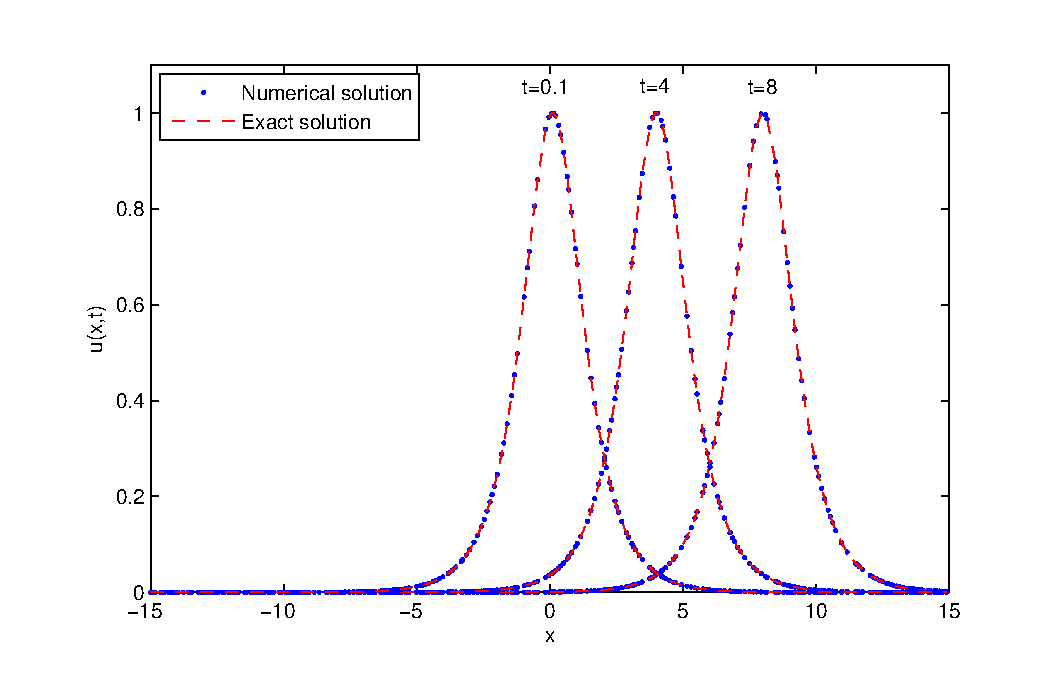
\includegraphics[height=7cm]{figure21.eps}} \caption{
جواب دقیق و تقریبی حاصل از روش باز تصویر به ازای 250 نقطه با توزیع هالتن و 
$\varepsilon=1$ } 
\label{fig:randpo}
\end{figure}
%
%
\begin{figure}
\centerline{
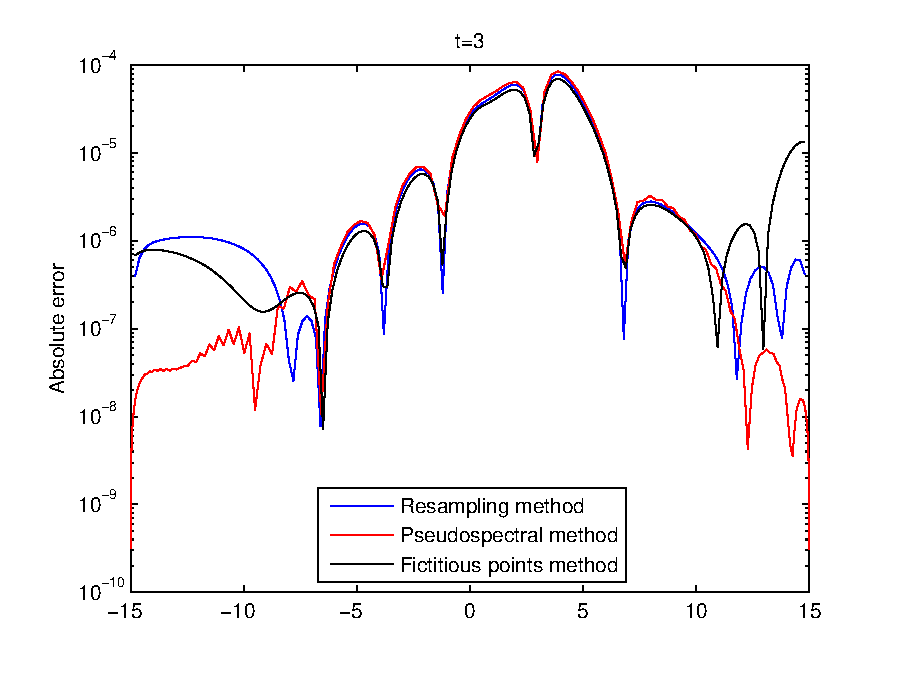
\includegraphics[height=6.5cm]{figure22.eps}
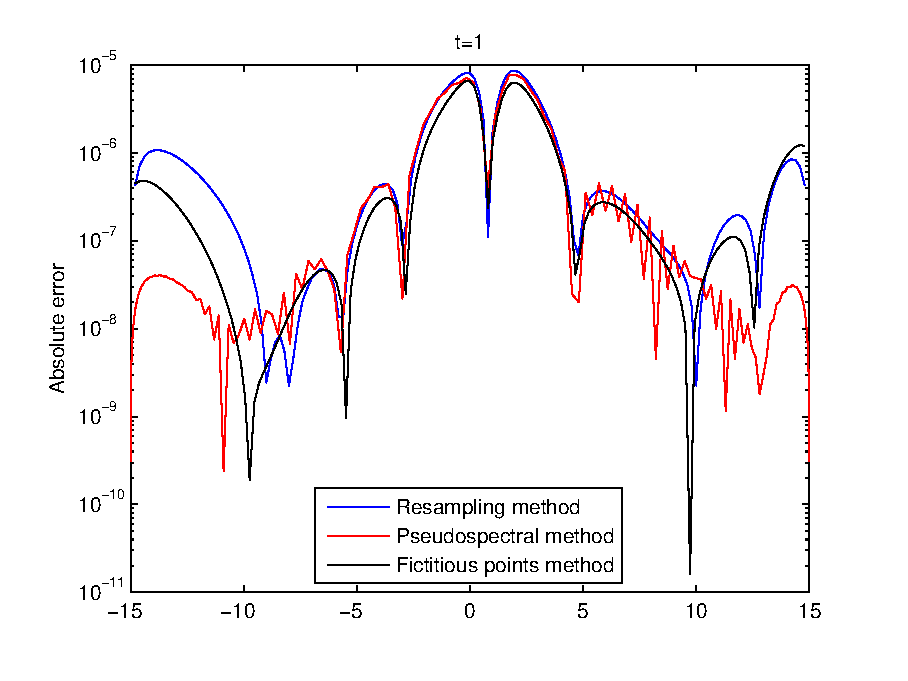
\includegraphics[height=6.5cm]{figure23.eps}} \caption{
مقایسه خطای مطلق روش باز تصویر و نقطه تصوری به ازای 150 نقطه یکنواخت و روش باز تصویر طیفی به ازای 150 نقطه چبیشف در 
$t=1$
و
$t=3$} \label{fig:absolute}
\end{figure}
%
%
معادله توسیع یافته روزنا که در مراجع
\citep{Wendland,ItoToi}
بیان شده است را در نظر می‌گیریم.
\begin{align}
u_t+\frac{1}{2}u_{xxxxt}=g(u)_x,\label{eq:test}
\end{align}
که
$g(u)=10u^3-12u^5-\frac{3}{2}u$.
جواب دقیق معادله
(\ref{eq:test})
بصورت
$u(x,t)=\textrm{sech}(x-t)$
می‌باشد. شرایط اولیه به ازای 
$t=0$
را می‌توان از جواب دقیق استخراج کرد.
\begin{align*}
u(x,0)=\textrm{sech}(x),
\end{align*}
همچنین شرایط مرزی نیز بفرم زیر است.
\begin{align*}
u(-15,t)&=\textrm{sech}(-15-t),&u&(15,t)=\textrm{sech}(15-t),\\
u_x(-15,t)&=-\textrm{sech}(-15-t)\textrm{tanh}(-15-t),&u_x&(15,t)=-\textrm{sech}(15-t)\textrm{tanh}(15-t).
\end{align*}
%
\begin{table}
\caption{ جواب تقریبی اختیار فروش امریکایی با دو دارایی پایه ناهمبسته با توزیع یکنواخت نقاط به ازای
 $\varepsilon=1.5$}
\label{tab:uinpoint}
\[\begin{array}{l@{\hspace{1cm}}c@{\hspace{1cm}}c@{\hspace{1cm}}c@{\hspace{1cm}}c}
\hline\noalign{\smallskip}
P(S_1,S_2,t) & 16 \times 16 \textrm{نقطه} & 21\times 21 \textrm{نقطه}
 & 31\times 31 \textrm{نقطه} & 41\times 41 \textrm{نقطه}  \\
\noalign{\smallskip}\hline\noalign{\smallskip}
  P(0.9,1,0)  & 7.8159e-002    & 7.4866e-002      &   7.6398e-002  &   7.5920e-002 \\
  P(1,0.9,0)  & 6.6373e-002    & 6.1842e-002      &   6.3400e-002  &   6.3700e-002 \\
  P(1,1.1,0)  & 3.1793e-002    & 3.1154e-002      &   3.2290e-002  &   3.2042e-002  \\
  P(1.1,1,0)  & 2.5447e-002    & 2.5159e-002      &   2.5865e-002  &   2.5925e-002 \\
\noalign{\smallskip}\hline
 \end{array}\]
\end{table}


\begin{table}
\centering{\caption{
خطای
$L_{\infty}$
حاصل از روش باز تصویر و نقطه تصوری به ازای 150 نقطه با توزیع یکنواخت و
$\varepsilon=0.5$
و خطای 
$L_{\infty}$
حاصل از روش باز تصویر طیفی به ازای 150 نقطه چبیشف
}}\label{tab:re1}
\vspace{-0.3cm}\begin{eqnarray*}\hspace{-0.2cm}\begin{array}{|c|c|c|c|c| } 
\hline {\rm \text{t} } &\hspace{2cm} {\rm
\text{باز‌تصویر}}
 &\hspace{2cm} {\rm \text{نقطه‌تصوری}} &\hspace{2cm} {\rm \text{باز‌تصویر‌طیفی}}\\
\hline
  0.1        &\hspace{2cm} 4.7842E^{-6}       &\hspace{2cm} 2.9565E^{-6}    &\hspace{2cm} 4.5572E^{-6}         \\
  0.5        &\hspace{2cm} 5.4018E^{-6}       &\hspace{2cm} 4.7338E^{-6}    &\hspace{2cm} 4.5603E^{-6}         \\
  1          &\hspace{2cm} 8.7933E^{-6}       &\hspace{2cm} 6.9239E^{-6}    &\hspace{2cm} 7.6580E^{-6}         \\
  3          &\hspace{2cm} 8.1032E^{-5}       &\hspace{2cm} 7.3506E^{-5}    &\hspace{2cm} 8.4876E^{-5}         \\
  5          &\hspace{2cm} 2.6041E^{-4}       &\hspace{2cm} 2.4963E^{-4}    &\hspace{2cm} 2.8425E^{-4}         \\
  8          &\hspace{2cm} 6.9731E^{-4}       &\hspace{2cm} 2.0524E^{-3}    &\hspace{2cm} 7.8322E^{-4}         \\
  10         &\hspace{2cm} 1.0868E^{-3}       &\hspace{2cm} 1.5169E^{-2}    &\hspace{2cm} 1.2464E^{-3}        \\
  \hline
 \end{array}\end{eqnarray*}
\end{table}

\begin{table}[htp] 
\centering\caption{
خطای
$L_{\infty}$
حاصل از روش باز تصویر و نقطه تصوری به ازای 150 نقطه با توزیع یکنواخت و
$\varepsilon=0.5$
و خطای 
$L_{\infty}$
حاصل از روش باز تصویر طیفی به ازای 150 نقطه چبیشف
}
\label{tab:re1}
\renewcommand*{\arraystretch}{1.2}
\vspace*{.4cm}
%\begin{LTR}
\begin{tabular}{||c|c|c|c||}%{|c@{\hspace{10mm}}|c@{\hspace{10mm}}|c@{\hspace{10mm}}|c@{\hspace{10mm}}|}
%{||c|c|c|c||}
\hline
$t$ & باز تصویر &  طیفی  & باز تصویر طیفی   \\
\hline
0.1     & 4.7842   & 2.9565     & 4.5572        \\
  0.5        & 5.4018       & 4.7338    & 4.5603        \\
  1          & 8.7933      &6.9239     & 7.6580        \\
  3          & 8.1032       & 7.3506   & 8.4876       \\
  5          & 2.6041      &2.4963    & 2/8425        \\
  8          &6.9731     & 2.0524     & 7.8322       \\
  10         & 1.0868      & 1.5169     & 1.2464      \\
\hline
\end{tabular}
%\end{LTR}
\end{table}
%
%
